\chapter{Reporting Power Values \normalsize{(Detailed Information)}}
\label{sec:reporting}

\noindent
This section describes the information that must be included with a power measurement submission. It also describes some optional information that submitters may decide to include.
\wl

\noindent
The section contains definitions of the terms used to describe the elements of a power submission, some background information, motivation about why the list contains the elements it does, and any other details that may be helpful.
\noindent


\section{Measuring Device Specifications}
\label{sec:MDSpecs}
\noindent
Measuring devices must meet the Level requirements as defined in 
Sections~\ref{sec:AQLevels} and \ref{sec:A1GTRM}. This section defines meter accuracy requirements.
\wl

\noindent
For Level 3, it is required to use any revenue grade meter, any meter accepted by spec power, or any meter documented to have an accuracy of 1\% or better. 
Revenue grade meters are defined by ANSI C12.20.  
Level 2 requires a meter with a minimum documented accuracy of 2\%.
Level 1 requires a meter with a minimum documented accuracy of 5\%.
\wl

\noindent
Also, refer to 
the {\itshape Power and Temperature Measurement Setup Guide \/} and the list of accepted power measurement devices from the Standard Performance Evaluation Corporation.
\wl

\noindent
\url{http://www.spec.org/power_ssj2008/}

\noindent
\url{http://www.spec.org/power/docs/SPECpower-Device_List.html }

\section{Measuring Device Terminology}
\label{sec:MDTerm}
\noindent
Levels 1 and 2 specify power measurements. Level 3 specifies an energy measurement, but reports a power value.

\subsection{Sampling}
\noindent
For Levels 1 and 2, power measurements must be sampled at least once per second. The actual measurements that constitute a sample may be taken much more frequently than once per second. 
\wl

\noindent
Sampling in an AC context requires a measurement stage that determines the true power delivered at that point and enters that value into a buffer where it is then used to calculate average power over a longer time.  So ``sampled once per second'' in this context means that the times in the buffer are averaged and recorded once per second.
Sampling delivered electrical power in a DC context refers to a single simultaneous measurement of the voltage and the current to determine the delivered power at that point.  The sampling rate in this case is how often such a sample is taken and recorded internally within the device.  
\wl

\noindent
If the submitter is sampling in a DC context, most likely it will be necessary to adjust for power loss in the AC/DC conversion stage. 
Refer to Section~\ref{sec:A3SIiIP} Aspect 3: Subsystems Included in Instrumented Power for details.

\subsection{Power-Averaged and Total Energy Measurements}
\label{sec:PAaTEM}
\noindent
The reported power values for Levels 1 and 2 are power-averaged measurements. A power-averaged measurement is one taken by a device that samples the instantaneous power used by a system at some fine time resolution for a given interval. The power-averaged measurement for the interval is the numerical average of all the instantaneous power measurements during that interval and constitutes one reported measurement covering that interval. 
\wl

\noindent
Consider Level 1, which requires only one reported power value. 
This reported power value may consist of several power measurements taken at a constant frequency of at least once per second and averaged over an interval. 
That interval must cover the entire core phase of the run which must be at least one minute long (see \ref{sec:core_phase} for definition of core phase).
For example, if power measurements may be taken once per second for one minute for a total of 60 power measurements and then averaged, Level 1 reports one power-averaged value.
\wl

\noindent
Level 2 also requires that power measurements be taken at a constant frequency at least once per second.
Level 2 requires that power values be reported for both the core phase of the workload and the total workload.
The reported power value for the core phase must be the result of at least 10 power measurements.
These 10 power measurements may themselves be power-averaged measurements.
Each of the required equally spaced measurements required for L2 must power-average over the entire separating space.  
\wl

\noindent
All the values reported by the meter must be used in the calculation.
\wl

\noindent
For example, the meter may sample at one-second intervals and report a value every minute. Assume that the core phase is 600 minutes long. Assume further that the requirement for 10 equally spaced measurements can be satisfied with 10 measurements spaced 50 minutes apart. Using just those 10 measurements does not conform to this specification because all the values reported by the meter during the core phase are not used. 
\wl

\noindent
Although those two measurements were equally spaced over 500 minutes , each averaged only over a minute. So some (the majority) of the separating space between the measurements was not included in the average. 
\wl

\noindent
For Levels 1 and 2, the units of the reported power values are watts.
\wl

\noindent

Level~3 specifies a total energy measurement that, when divided by the measured time, also reports power. An integrated measurement is a continuing sum of energy measurements. Typically, there are hundreds of measurements per second.  Depending on the local AC power line frequency, there must be at least 120 or 100 measurements per second. The measuring device samples voltage and current many times per second and integrate those samples to determine the next total energy consumed reading. 
\wl

\noindent
Level 3 reports an average power value for the core phase, an average power value for the whole run, at least 10 equally spaced energy values within the core phase, and the elapsed time between the initial and final energy readings in the core phase. The average power value for the core phase is the difference between the initial and final energy readings divided by the elapsed time.

\section{Aspect and Quality Levels}
\label{sec:AQLevels}
\noindent
Table~\ref{tab:levels} summarizes the aspect and quality levels introduced in Section~\ref{sec:intro} Introduction

%INSERT TABLE 1
\noindent
\begin{table}
\caption{Summary of aspects and quality levels}
\label{tab:levels}
\begin{tabular}{|p{3.0cm}|p{3.5cm}|p{3.5cm}|p{3.5cm}|} \hline
\textbf{Aspect}&\textbf{Level 1}&\textbf{Level 2}&\textbf{Level 3}\\ \hline

\textbf{1a:~Granularity} &
One power sample per second &
One power sample per second &
Continuously integrated energy\\
\hline


\textbf{1b:~Timing} &
The entire core phase of the run, at least one minute &
Equally spaced across the full run &
Equally spaced across the full run   \\
\hline

\textbf{1c:~Measurements} &
Core phase average power &
$\bullet$ 10 average power measurements in the core phase &
$\bullet$  10 energy measurements in the core phase\\

 & &
$\bullet$  Full run average power &
$\bullet$  Full run average power \\

 & &
$\bullet$  idle power &
$\bullet$  idle power \\
\hline

\textbf{2: Machine \newline fraction}  &
The greater of 1/10 of the compute subsystem or 2 kW  &
The greater of 1/8 of the compute-node subsystem or 10 kW  &
The whole of all included subsystems \\
\hline

\textbf{3:~Subsystems} &
Compute-nodes and measured or estimated interconnect &
All participating subsystems, either measured or estimated &
All participating subsystem must be measured \\
\hline

\textbf{4: Point of measurement} &
Upstream of power conversion &
Upstream of power conversion &
Upstream of power conversion\\

 &
\centering \textbf{OR} &
\centering \textbf{OR} &
\centering \textbf{OR} \tabularnewline

 &
Conversion loss modeled with manufacturer data &
Conversion loss modeled with off-line measurements of a single power supply &
Conversion loss measured simultaneously \\
\hline
\end{tabular}
\end{table}

\section{Aspect 1: Granularity, Timespan and Reported Measurements}
\label{sec:A1GTRM}
\noindent
Aspect 1 has the following three parts. Levels 1, 2, and 3 satisfy this aspect in different ways.

\begin{itemize}
\item
The granularity of power measurements. This aspect determines the number of measurements per time element.
\item
The timespan of power measurements. This aspect determines where in the time of the workload's execution the power measurements are taken.
\item
The reported measurements. This aspect describes how the power measurements are reported.
\end{itemize}

\noindent
For all required measurements, the submission must also include the data used to calculate them. For Level 2 and Level 3 submissions, the supporting data must include at least 10 equally spaced points in the core of the run. 
\wl

\noindent
Levels 2 and 3 require a number of equally spaced measurements to be reported for two reasons.  

\begin{itemize}
\item
One is that facility or infrastructure level power measurements are typically taken by a system separate from the system OS and thus cannot be easily synchronized with running the benchmark.  
\item
Secondly, with multiple periodic measurements, more reporting points are included before and after the benchmark run to ensure that a uniform standard of "beginning" and "end" of the power measurement can be applied to all the power measurements on a list.  
\end{itemize}

\noindent
There is no maximum number of reported points, although one reported measurement per second is probably a reasonable upper limit. The submitter may choose to include more than 10 such points.
\wl

\noindent
The number of reported average power measurements or total energy measurements is deliberately given large latitude.  Different computational machines will run long or short benchmark runs, depending on the size of the machine, the memory footprint per node, as well as other factors.  Typically the power measurement infrastructure is not directly tied to the computational system's OS and has its own baseline configuration (say, one averaged measurement every five minutes).  These requirements are specified not only to give a rich data set but also to be compatible with typical data center power measurement infrastructure.
\wl

\noindent
All levels specify that power measurements be performed within the core phase of a workload. Levels 2 and 3 specify that a power measurement for the entire application be reported. Consequently, these levels require measurements during the run but outside of the core phase.

\subsection{Core Phase}
\label{sec:core_phase}
\noindent
All submissions must include the average power within the core (parallel computation) phase of the run. 
\wl

\noindent
In order to correlate the power measurement and the performance measurement to obtain the power efficiency, power and performance must be measured over the exact same time period.
Therefore, the core phase is defined as the time period that is used for the performance calculation.
\wl

\noindent
For example, the core phase of the Linpack workload is the portion of the code that actually solves the matrix.
It is the numerically intensive solver phase of the calculation.
In case of the standard HPL implementation of the Linpack benchmark as provided by netlib.ork (\url{http://www.netlib.org/benchmark/hpl/}) this is the time spent in the routing {\ttfamily HPL\_pdgesv}.
Note that HPL as of version 2.1 contains a timer routine that prints start and end time of the core phase to facilitate power measurements, which looks like:\newline
{\ttfamily
HPL\_pdgesv() start time Wed Jun 30 21:49:08 2015\newline
HPL\_pdgesv() end time Wed Jun 30 22:23:15 2015
}.

\subsection{The Whole Run}
\noindent
Level 2 and Level 3 submissions must also include the average power for the whole run, from the initiation of the job to its completion. 
\wl

\noindent
Since HPL only reports the time spent executing the core phase of the workload, the time for the total run must be measured and reported separately by the submitter, for example by prepending the UNIX time command to the job invocation or the parallel application launch, whichever is earlier.
\wl

\noindent
Levels 2 and 3 require the entire run to be measured and reported because HPL (the default workload at the time this document was written) drops significantly in power consumption during the course of a computation, as the matrix size being computed gets smaller.  Requiring the entire run eliminates systematic bias caused by using different parts of the run for the measurement. Figure~\ref{fig:powprof} shows an example of a power graph taken from an HPL run on the LLNL Muir system in the fall of 2011.
\wl

\noindent
Note that the power drops by 8\% or so during the computational phase of the run.  This graph also illustrates the need for the device measurement to have as high a time resolution as possible.  The spread of power measurements even within a small time span is very likely caused by the sampling going in and out of phase with the AC input power. Figure~\ref{fig:sopm} shows a smaller time slice that clearly illustrates this.
\wl


%INCLUDE FIG 3-1
\begin{figure}
\centering
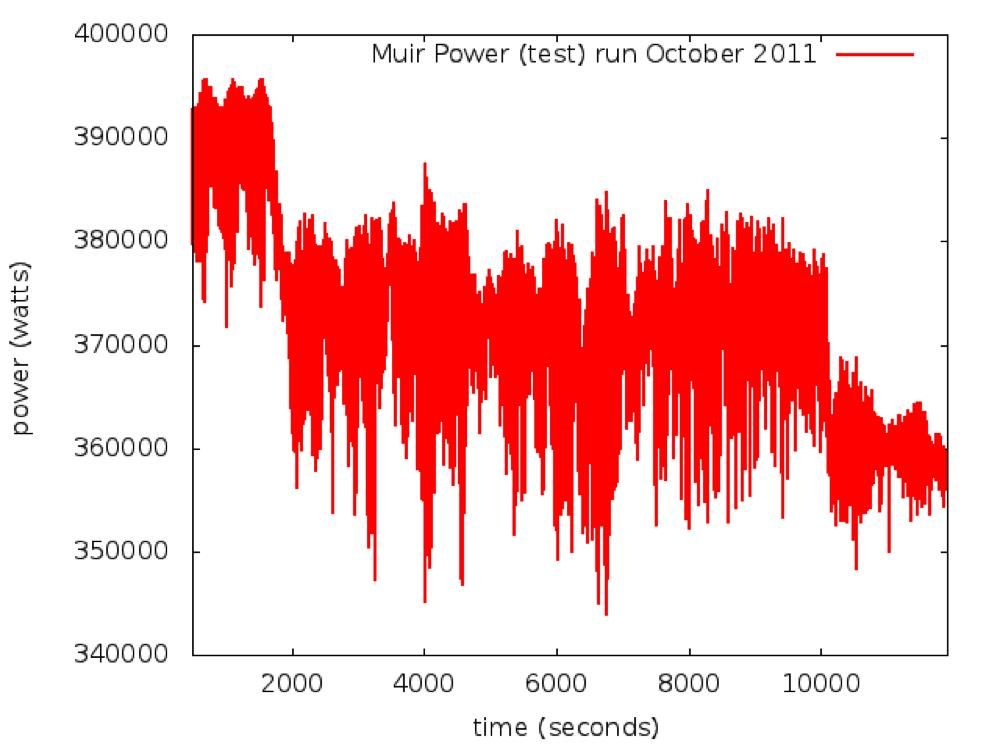
\includegraphics[width=4in]{fig3-1}
\caption{Power Profile HPL Run}
\label{fig:powprof}
\end{figure}

%INCLUDE FIG 3-2
\begin{figure}
\centering
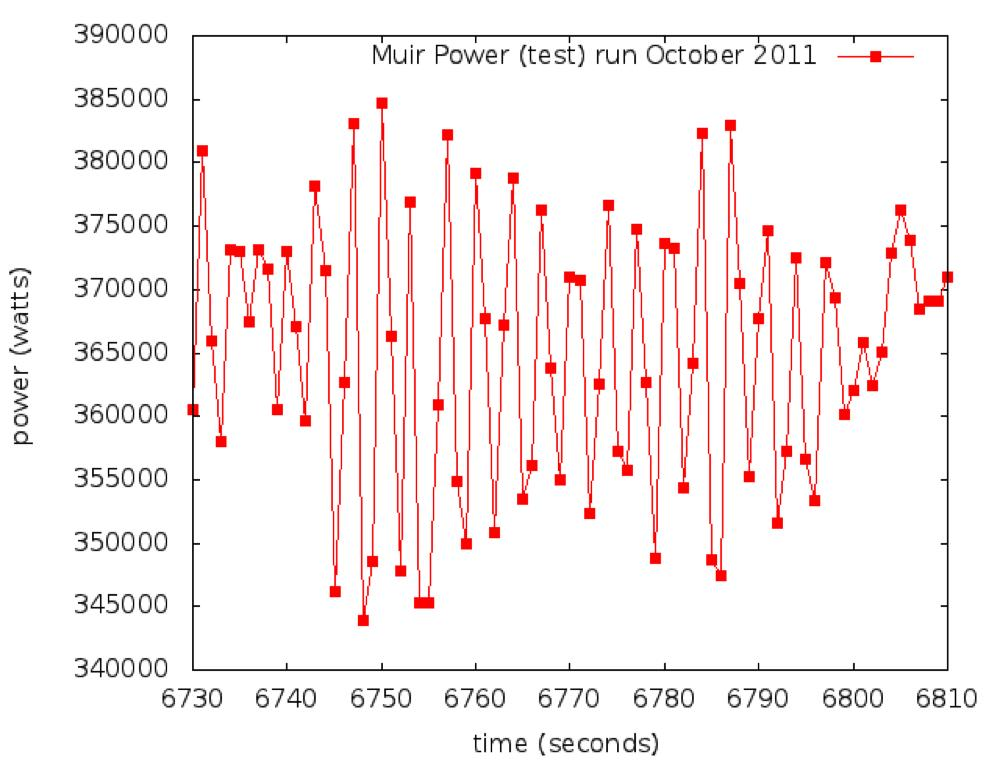
\includegraphics[width=4in]{fig3-2}
\caption{Spread of Power Measurements}
\label{fig:sopm}
\end{figure}

\noindent
The boxes are individual one-second power samples.  This fast up-down fluctuation is not caused by the behavior of an individual power supply; the power being sampled is over the entire computer system doing the HPL run.  The reason that L3 requires integrating total energy meters is because they measure at a high enough frequency to not be subject to these sampling artifacts.
\wl

\noindent
L2 and L3 each decrease the device's inherent time measurement granularity.  L2 allows 1-second intervals of the input power.  L3 requires an integrating total-energy meter, which samples the input power multiple times per AC cycle and so is much less susceptible to sampling artifacts caused by the AC waveform.  

\subsection{Level 1}
\noindent
The device measurement granularity must be at least one instantaneous measurement of power per second. This requirement holds whether the measurement is DC or AC.
\wl

\noindent
There must be at least one power-averaged measurement during the run.
The total interval covered must be the core phase of the run which must be at
least one minute long.
\wl

\noindent
Figure~\ref{fig:a1l1pm} illustrates Aspect 1 Level 1 power measurement. If, as required, the instantaneous measurement must be at least once per second and you are measuring for one minute, you have taken at least 60 instantaneous measurements and averaged them.

%INCLUDE FIG 3-3
\begin{figure}
\centering
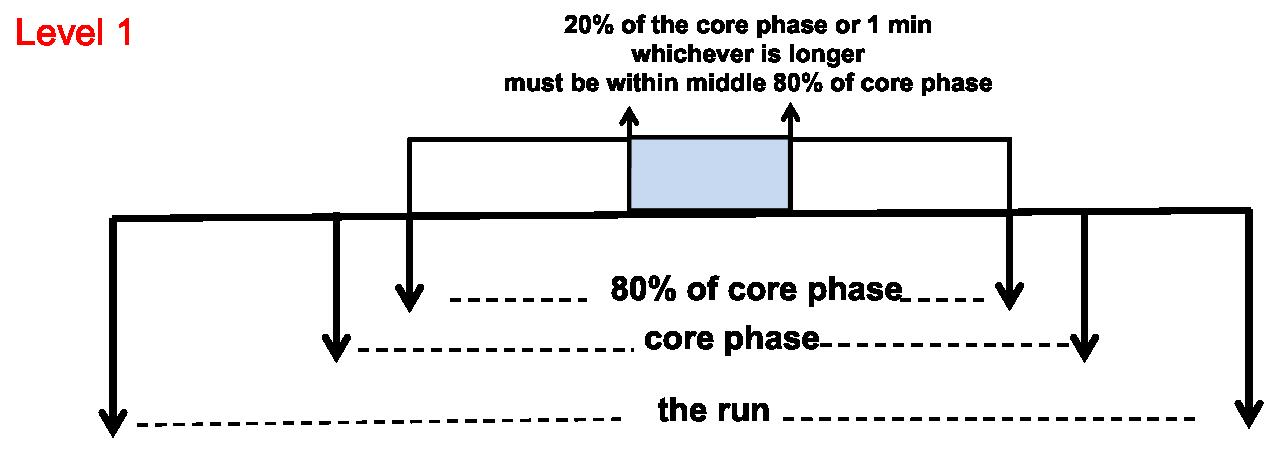
\includegraphics[width=4in]{fig3-3}
\caption{Aspect 1 Level 1 Power Measurements}
\label{fig:a1l1pm}
\end{figure}

\subsection{Level 2}
\noindent
Level 2 submissions include a measurement of the average power during the core phase of the run and the average power during the full run. The workload run must have a series of equally spaced power-averaged measurements of equal length. These power-averaged measurements must be spaced close enough so that at least 10 measurements are reported during the core phase of the workload. The reported average power for the core phase of the run will be the numerical average of the 10 (or more) power-averaged measurements collected during the core phase.  
\wl

\noindent
The complete set of power-averaged measurements used to calculate average power must also be provided.
The device measurement sampling granularity must be at least one instantaneous measurement of power per second.
\wl

\noindent
There is some unspecified number of power-averaged measurements during the workload but outside of the core phase. The reported average power for the whole run will be the numerical average of the power measurements for the whole run.  
\wl


\noindent
Figure~\ref{fig:a1l2pm} illustrates Aspect 1 Level 2 power measurement. Each measurement is an average of instantaneous power measurements, and these instantaneous measurements are taken once per second. As an example, the figure shows 10 power-averaged measurements within the core phase and four power-averaged measurements outside the core phase, two before the core phase and two after the core phase.

%INCLUDE FIG 3-4
\begin{figure}
\centering
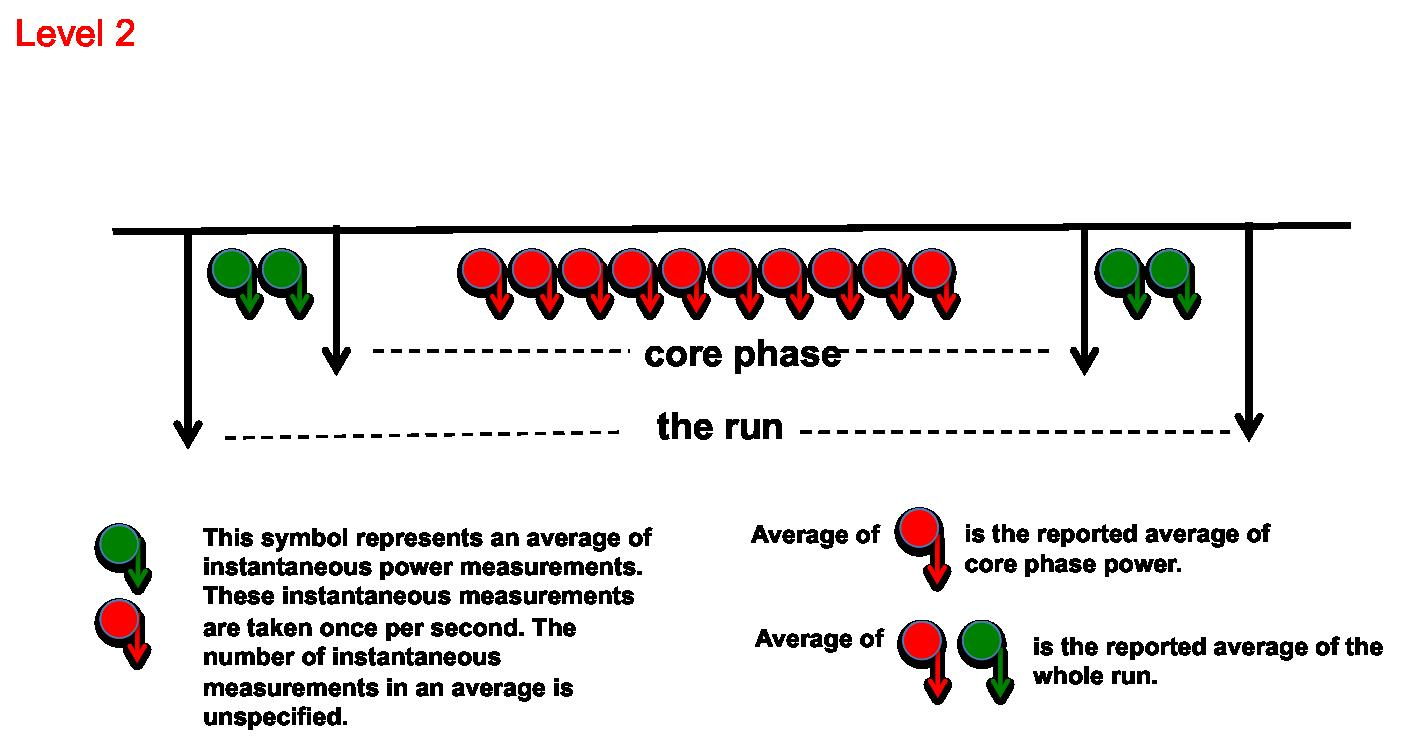
\includegraphics[width=4in]{fig3-4}
\caption{Aspect 1 Level 2 Power Measurements}
\label{fig:a1l2pm}
\end{figure}

\subsection{Level 3}
\noindent
Level 3 submissions include a measurement of the average power during the core phase of the run and the average power during the full run.
\wl

\noindent
The complete set of total energy readings (at least 10 during the core computation phase) must be included, along with the execution time for the core phase and full run. 
\wl

\noindent
Level 3 requires continuously integrated total energy measurements rather than power-averaged measurements. The readings must begin before the start of the run and extend to when it is finished.
\wl

\noindent
The measuring device must sample voltage and current, whether AC or DC, at least 120 times or 100 times per second (depending on the local AC power line frequency) and integrate those samples to determine the next total energy consumed reading.  Sampling at a greater rate is permitted. 
\wl

\noindent
The reported total energy readings must be spaced so that at least 10 reported readings fall within the core phase of the workload. Note that each reported reading is the average of many samples.
\wl


\noindent
Figure~\ref{fig:a1l3pm} illustrates Aspect 1 Level 3 power measurement. The figure shows 10 readings in the core phase of the workload. Note that these are integrated readings.  To obtain a power reading, one must subtract two integrated readings and divide by the time between the readings.

%INCLUDE FIG 3-5
\begin{figure}
\centering
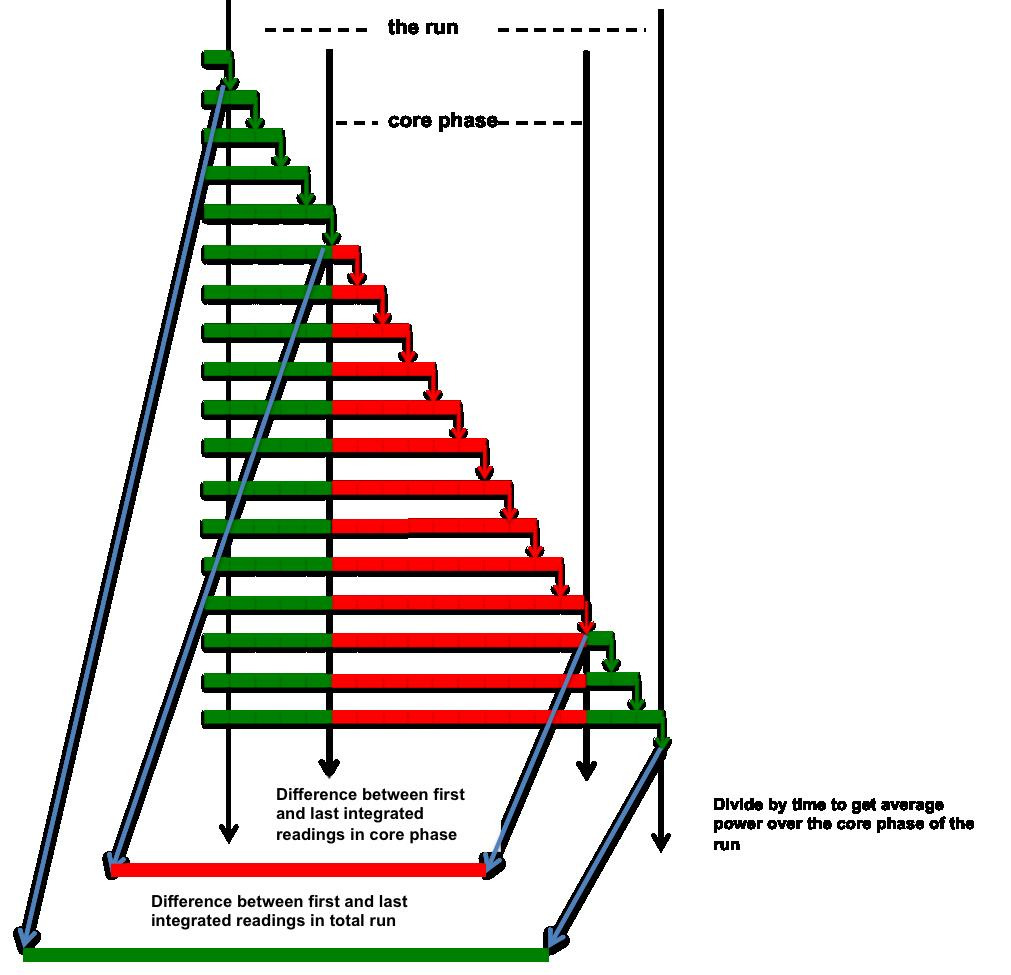
\includegraphics[width=4in]{fig3-5}
\caption{Aspect 1 Level 3 Power Measurements}
\label{fig:a1l3pm}
\end{figure}

\section{Format of Reported Measurements}
\label{sec:FoRM}
\noindent
Levels 2 and 3 require the complete set of measurements. The submitter may choose to provide these values in a CSV file. Do not provide scans of paper documents.
\wl

\noindent
The submitter may find it useful to create a graph showing the power and energy during the workload as shown in Figure~\ref{fig:powengwl}. Keep this graph for reference, but do not provide it as part of the submission.


%INCLUDE FIG 3-6
\begin{figure}
\centering
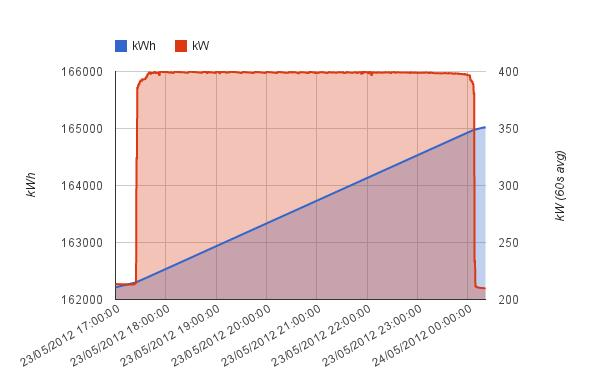
\includegraphics[width=4in]{fig3-6}
\caption{Power and Energy During the Workload}
(used with permission from Universit‚ Laval, Calcul Qu‚bec, Compute Canada)
\label{fig:powengwl}
\end{figure}

\section{Aspect 2: Machine Fraction Instrumented}
\label{sec:A2MFI}
\noindent
Aspect 2 specifies the fraction of the system whose power feeds are instrumented by the measuring equipment. 
\wl

\noindent
Level 3 requires that the entire machine be measured. Level 2 requires a higher fraction than Level 1.
\wl

\noindent
When calculating the average power of the full machine for Levels 1 and 2, the measured power must be divided by this fraction to 
estimate the average power drawn by the whole machine. For example, if the submitter measures the power delivered 
to $ \frac{1}{4} $ of the machine, the submitter must then multiply the measured power by 4 to estimate power for the whole machine.  
The higher machine fractions are required at the higher quality levels to reduce the effects of random fluctuations and minor differences in hardware influencing the power measurements.  The larger the sample, the more transients will tend to cancel out.
\wl

\noindent
The requirements for each quality level are as follows.

\begin{itemize}
\item
L1: $ \frac{1}{64} $ of the compute-node subsystem or 1 kW, whichever is greater
\item
L2: $ \frac{1}{8} $ of the compute-node subsystem or at least 10 kW, whichever is greater
\item
L3: the power use of the whole machine must be measured
\end{itemize}

\section{Aspect 3: Subsystems Included in Instrumented Power}
\label{sec:A3SIiIP}
\noindent
Aspect 3 specifies the subsystems included in the instrumented power. 
\wl

\noindent
Subsystems in the context of this document are power subsystems. A power subsystem is that part of a supercomputer which can be measured in isolation for power consumption while the supercomputer is performing a task. 
\wl

\noindent
Subsystems include computational nodes, any interconnect network the application uses, any head or control nodes, any storage system the application uses, and any internal cooling devices (self-contained liquid cooling systems and fans).
\wl

\noindent
If some subsystems are part of the measured power, their power may not be subtracted out after the fact.  The explicitly measured value must be used as is.
\wl


\noindent
For Level 1, both the compute-node subsystem and the interconnect must be reported.  
The compute-node subsystem power must be measured. 
The interconnect subsystem participating in the workload must also be measured or, if not measured, the contribution must be estimated.
Include everything that you need to operate the interconnect network that is not part of the compute subsystem. 
This may include infrastructure that is shared, but excludes that part that is not servicing the current cluster.
For some systems, it may be impossible not to include a power contribution from some subsystems. 
In this case, provide a list of the measured subsystems, but do not subtract an estimated value for the included subsystem. 
\wl

\noindent
For Level 2,  include the compute node subsystem. Other subsystems participating in the workload must be measured or estimated. The estimations must be based on derived numbers from the equipment manufacturer's specifications. 
\wl


\noindent
For Level 3, all power going to the parts of a computer system that participate in a workload must be included in the power measurement. 
\wl

\noindent
For Level 3, the reported power measurement must include all computational nodes, any interconnect network the application uses, any head or control nodes, any storage system the application uses, all power conversion losses inside the computer, and any internal cooling devices (self-contained liquid cooling systems and fans).  
\wl

\noindent
For Levels 2 and 3, the reported power measurement may exclude storage subsystems that don't participate in the workload. It is not required to exclude such storage subsystems. However, if these storage subsystems are part of the cabinet or rack being measured, they may not be excluded even if they are not used. That is, the submitter cannot calculate their contribution and subtract that contribution. If the storage subsystem is not part of the rack or cabinet being measured and it does not participate in the workload, it need not be measured.
\wl

\noindent
In some cases, the submitter may be measuring power that the application doesn't actually use. If the submitter can exclude the unused subsystems from the measurement or easily turn off the power to the unused subsystems, then the submitter can choose not to include those subsystems in the measurement. 
\wl

\noindent
For example, the node board may include compute nodes and GPUs, and the application may not actually use the GPUs.  If you cannot easily shut down the GPUs (say with an API), you must still include the power that they use. It is not acceptable to measure the power for both the compute nodes and the GPUs and then subtract the GPU power from the measurement.
\wl

\noindent
A site may include more subsystems than are strictly required if it chooses or if it is advantageous from a measurement logistics point of view.  
\wl

\noindent
A particular system may have different types of compute nodes. The system may have compute nodes from different companies or even compute nodes with different architectures. These compute nodes are said to belong to different heterogeneous sets.
\wl

\noindent
With Level 3, the submitter need not be concerned about heterogeneous sets of compute nodes because Level 3 measures the entire system. 
\wl

\noindent
Levels 1 and 2, however, measure a portion of the compute-node subsystem and estimate contributions from unmeasured portions. With Levels 1 and 2, the submitter must measure at least one member of each heterogeneous set. The submitter must include a power measurement from at least one compute node in each heterogeneous set and then estimate the contribution from the remaining members of the set. 
\wl

\noindent
For example, assume there exist two sets of compute nodes, a set called A and another called B.  The submitter is able to measure the power 
consumed by $ \frac{1}{2} $ of the A compute nodes and $ \frac{1}{4} $ of the B compute nodes.
\wl

\noindent
The total power measurement reported for compute nodes would then be 

\noindent
\[ Total~power=2*(power~from~compute~nodes~A) 
                              + 4*(power~from~compute~nodes~B) \]

\noindent
The assumption of Levels 2 and 1 is that all the compute nodes in a set react identically to the workload.


\section{Aspect 4: Point where the Electrical Measurements are Taken}
\label{sec:A4wEMaT}
Aspect 4 specifies where in the power distribution system the power delivery is measured.  For all quality levels, the submission indicates where power is measured and the quantity of parallel measurements points.
\wl

\noindent
Measurements of power or energy are typically made at multiple points in parallel across the computer system. For example, such locations can be at the entrance to each separate rack, or at the exit points of multiple building transformers. 
\wl

\noindent
All the reported measurements taken in parallel at a given instant in time are then summed into a total measurement for that time.  The total measurement for a given moment in time constitutes one entry in the series of measurements that becomes part of the submission.
\wl

\noindent
AC measurements are upstream of the system's power conversion. If the measurements are in a DC context, the submitter may have to take into account some power loss. 
Refer to Section~\ref{sec:AfPL} Adjusting for Power Loss.
\wl

\noindent
Electrical power or energy measurements shall be taken in one of the following locations.

\begin{itemize}
\item[{A)}]
At a point upstream of where the electrical supply from the data center is delivered to the computer system

OR

\item[{B)}]
At the point of the electrical supply delivery to the computer system from the data center

OR

\item[{C)}]
At a point just inside of the computer system that is electrically equivalent to location B) above.  This includes the following. 

\begin{itemize}
\item
At any point within a passive PDU, at the input to the PDU, at the exit point(s) of the PDU, or anywhere in between 
\item
At the entry point to the first power-modifying component (for example, the Blue Gene bulk power module, Cray AC/DC converters, and possibly the input point to one or more crate power supplies)
\end{itemize}
\end{itemize}

\noindent
If the measuring device or devices used to satisfy Aspect 1 also meet the ABC location requirements specified above, then those devices are sufficient to obtain the measurements needed for submission.

\subsection{Adjusting for Power Loss}
\label{sec:AfPL}
\noindent
If the measurement device(s) that satisfy Aspect 1 are downstream of the ABC locations specified above, then two sets of measurements must be taken in order to determine the power loss between the required and the actual measurement location. 

\begin{itemize}
\item
For a Level 1 measurement, the power loss may be a load-varying model based on specifications from the manufacturer.  
\item
For a Level 2 measurement, the power loss may be a load-varying model based on an actual physical measurement of one power supply in the system.  
\item
For a Level 3 submission, the power loss must be measured simultaneously by a device at the required point (one of the ABC locations) measured at least once every five minutes, averaged long enough to average out the AC transients. 
\end{itemize}

\noindent
For all three levels, the power losses used and how they were determined must be part of the submissions.

\subsection{Data Center Schematic}
\noindent
Figure~\ref{fig:powmeasschem} is an example of a simple power measurement schematic. This example shows only one power measurement point.
\wl


\noindent
Submitters may find it useful to create such a schematic to identify the power measurement locations. Keep this schematic for reference, but do not provide it as part of the submission.

%INCLUDE FIG 3-7
\begin{figure}
\centering
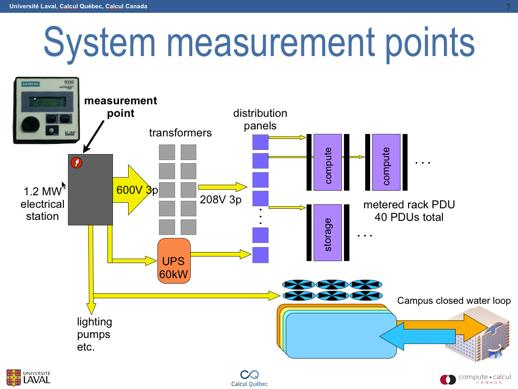
\includegraphics[width=4in]{fig3-7}
\caption{Example of a Power Measurement Schematic}
(used with permission from Universit‚ Laval, Calcul Qu‚bec, Compute Canada)
\label{fig:powmeasschem}
\end{figure}


\section{Environmental Factors}
\label{sec:EF}
\noindent
Reporting information about the cooling system temperature is optional.
It is requested to provide a description of the cooling system as well as where and how the temperature was measured.
Reporting temperature allows for better comparison of reported results, as there is a indirect correlation between temperature and power.

\wl

\noindent
All other environmental data is optional. 
Other environmental data may include factors such as:

\begin{packed_item}
\item[{-}]
\% deviation between supply and rated voltage and frequency (recommended +/-5\%)
\item[{-}]
\% total harmonic distortion (recommended \textless 2\% THD )
\item[{-}]
line impedance (recommended \textless 0.25 ohm)
\item[{-}]
relative humidity
\end{packed_item}

